% \documentclass[sigconf]{acmart}
\documentclass[anonymous, sigconf]{acmart}
\settopmatter{printacmref=true}

\AtBeginDocument{%
  \providecommand\BibTeX{{%
    Bib\TeX}}}

% 清除所有会议/版权信息
\setcopyright{none}
\copyrightyear{}
\acmDOI{}
\acmConference[]{}{}{}
\acmISBN{}

% 移除页脚横线（关键！）
\renewcommand{\footnoterule}{}

\usepackage{doi}

\begin{document}

\title{ZhuLong: An Execution-Grounded LLM Agent for EDA Scripting}

\author{Yang Liu}
\email{paul.liu@cxmt.com}
\author{Shiwei Hou}
\email{shiwei.hou@cxmt.com}
\author{Xiyuan Chen}
\email{chenxiyuan@mail.ustc.edu.cn}
\author{Yu Wang}
\author{Sen Yuan}
\author{Qirui Gan}
\author{Shao You}
\author{Feifan Chen}
\author{Wencheng Li}
\author{Shuyang Hu}
\author{Yongzhou Liu}
\author{Emma Xia}
\author{Xiaojing Lu}
\author{Hao Wang}
\author{Fan Xu}
\author{Yanfeng Li}
\affiliation{%
  \institution{Changxin Memory Technologies, Inc.}
  \country{China}
}


\renewcommand{\shortauthors}{Liu et al.}

%%
%% The abstract is a short summary of the work to be presented in the
%% article.
\begin{abstract}
    EDA scripting with tool-specific, often undocumented APIs remains a long-tail 
    bottleneck that existing LLM-based tooling fails to address. This paper presents 
    \textbf{ZhuLong}, an execution-grounded LLM coding agent for PyAether, SKILL, and Tcl 
    that combines API retrieval, documentation inspection, and sandbox execution via 
    unified MCP tools into a closed generate--execute--refine loop. We further provide 
    a \textbf{theoretical grounding} for why runtime observation is necessary: EDA correctness 
    is a \emph{situated} property that cannot be guaranteed from static knowledge, 
    and we formalize this ``grounding gap'' with a Bayesian argument showing it is 
    bounded by observation fidelity---not model scale. The Harness supplies precisely 
    that observation, by reading the environment's documented API facts and by reading 
    back what executing code does to the live design.
    % 使用工具特定且常无文档的EDA API进行脚本编写，仍是现有LLM工具无法解决的长尾瓶颈。
    % 本文提出ZhuLong，一个面向PyAether和SKILL的执行驱动LLM代码智能体，通过统一MCP工具将
    % API检索、文档查阅和沙盒执行组合为"生成-执行-修正"闭环。我们进一步给出执行必要性的
    % 理论论证：EDA正确性是情境化属性，无法从静态知识保证；我们用贝叶斯论证形式化这一
    % "落地鸿沟"，说明它受观测保真度而非模型规模约束，沙盒执行正是弥合该鸿沟的观测通道。

    We evaluate ZhuLong on \textbf{EDA-Eval-PyAether}, a benchmark of 158 real-world 
    tasks with assertion-based execution, where the complete system achieves 
    \textbf{84.8\%} Pass@1 in the commercial Empyrean Aether environment, substantially 
    outperforming a pure LLM baseline (\textbf{11.4\%}). Ablation studies show the 
    execution loop is decisive: adding sandbox execution to retrieval yields +[TBD] pp, 
    while removing either execution ($-[TBD]$ pp) or retrieval ($-3.2$ pp) reduces 
    accuracy---consistent with the theoretical prediction. A complementary offline 
    \textbf{API self-exploration} mechanism contributes a further +[TBD] pp accuracy and 
    reduces per-task tool calls by 22.1\%; we report its scale, cost, and stopping 
    criteria in full.
    % 我们在EDA-Eval-PyAether（158个真实任务、断言式执行验证）上评估ZhuLong，完整系统在
    % 商业Empyrean Aether环境中达到84.8\%的Pass@1，显著优于纯LLM基线（11.4\%）。消融表明
    % 执行闭环是决定性的：在检索之上加入沙盒执行带来+[TBD]个百分点，而移除执行（-[TBD]pp）
    % 或检索（-3.2pp）都会使准确率坍塌——与理论预测一致。互补的离线API自探索机制进一步
    % 带来+[TBD]个百分点准确率与22.1\%的工具调用削减；我们完整报告其规模、成本与停止准则。
All quantitative results in this draft are provisional, obtained on the PyAether-only 
    slice; final numbers will be reported on the unified \textbf{EDA-Scripting-Bench} 
    (PyAether + SKILL + Tcl).
    % 本文所有定量结果为暂定值，均来自PyAether切片；最终结果将在统一评测集EDA-Scripting-Bench（PyAether + SKILL + Tcl）上报告。

\end{abstract}

\keywords{LLM Agents for EDA, EDA Scripting, Code Generation, Sandbox Execution, Execution Grounding}

\begin{CCSXML}
<ccs2012>
   <concept>
       <concept_id>10010583.10010682.10010712.10010715</concept_id>
       <concept_desc>Hardware~Software tools for EDA</concept_desc>
       <concept_significance>500</concept_significance>
   </concept>
 </ccs2012>
\end{CCSXML}
\ccsdesc[500]{Hardware~Software tools for EDA}

\maketitle

\section{Introduction}
\label{sec:introduction}

Large language models (LLMs) have demonstrated strong capabilities in general-purpose code generation \cite{vaswani2017attention, openai2023gpt4, yang2025qwen3}. However, applying LLMs to EDA scripting—where engineers routinely manipulate in-memory design databases, create layout instances, route schematics, and query netlists—remains challenging. First, EDA APIs are long-tailed and tool-specific; many rarely appear in public training corpora. Second, correctness cannot be verified statically: it depends on observable side effects in a real EDA environment, such as modified layouts or updated schematics. Third, without execution feedback, static generation cannot diagnose errors or iteratively refine incorrect code \cite{chen2024dawning, blocklove2024eda}. Existing LLM-based EDA work has mainly focused on HDL generation \cite{thakur2023verigen, liu2023rtlcoder}, while scripting with real tool APIs—especially with incomplete documentation and sandbox execution—remains underexplored.
% 大语言模型在通用代码生成方面表现强大，但应用于EDA脚本——工程师日常操作内存中的设计数据库、创建版图实例、布线原理图、查询网表——仍面临挑战。第一，EDA API具有长尾性和工具特定性，许多很少出现在公开训练语料中。第二，正确性无法静态验证：它取决于真实EDA环境中的可观察副作用，如版图修改或原理图更新。第三，没有执行反馈，静态生成无法诊断错误或迭代修正代码。现有LLM-for-EDA工作主要集中在HDL生成，而面向真实工具API、沙盒执行和不完整文档的脚本生成仍研究不足。

This paper presents \textbf{ZhuLong}, an execution-grounded LLM coding agent for PyAether, SKILL, and Tcl. Named after a mythical creature whose opened eyes bring light, ZhuLong aims to illuminate opaque EDA APIs and automate tool-specific scripting workflows. Built on Cline-CLI \cite{cline2024cline}, ZhuLong extends three MCP tools \cite{lee2025autoeda}—\texttt{search\_apis}, \texttt{get\_api\_details}, and \texttt{run\_code}—that form a closed loop: retrieve candidate APIs, inspect their documentation, execute code in the EDA environment with execution feedback, and iteratively refine based on observed errors or outputs. All tools accept a unified \texttt{lang} parameter, so the same agent logic covers PyAether, SKILL, and Tcl. To further address incomplete or outdated documentation, ZhuLong introduces an offline \textbf{API self-exploration mechanism} that proactively explores undocumented API behaviors in the sandbox via \textbf{counterfactual experimentation}---deliberately testing alternative parameter values, observing execution outcomes, inferring constraints and usage patterns, and storing the discovered information as enhanced API documentation for future queries. Beyond the engineering, we provide a \textbf{theoretical foundation} (Section~\ref{sec:grounding-theory}): EDA scripting correctness is a \emph{situated} property that cannot be guaranteed from static knowledge, and a Bayesian analysis shows the resulting ``grounding gap'' is bounded by observation fidelity---not model scale---explaining why runtime observation is essential, and why the Harness must supply both halves of it: reading the environment's documented API facts, and reading back what executing code does to the live design.
% 本文提出\textbf{ZhuLong}，一个面向PyAether和SKILL的执行驱动LLM代码智能体。其名源自中国神话中睁眼带来光明的神兽，寓意照亮不透明的EDA API并自动化工具特定的脚本流程。ZhuLong基于Cline-CLI构建，扩展三个MCP工具——\texttt{search\_apis}、\texttt{get\_api\_details}和\texttt{run\_code}——形成闭环：检索候选API、查阅文档、在沙盒EDA环境中执行代码、基于观察到的错误或输出迭代修正。所有工具接受统一的\texttt{lang}参数，以相同智能体逻辑同时支持PyAether和SKILL。为了进一步解决文档不完整或过时的问题，ZhuLong引入了离线\textbf{API自探索机制}，通过沙盒中的\textbf{反事实实验}主动探索未文档化的API行为——有意识地测试不同参数取值、观察执行结果、推断约束和使用模式、将发现的信息存储为增强的API文档供后续查询使用。

The main contributions are:

\begin{itemize}
    \item \textbf{An account of \emph{which} factor sets the ceiling, with measurements that distinguish them (RQ1).}
    We formalize the \emph{grounding gap}: EDA correctness is a situated (L4) property that no
    offline knowledge can guarantee, and a Bayesian argument shows the resulting gap is
    bounded by \emph{observation fidelity} rather than by the capacity of the model
    (Section~\ref{sec:grounding-theory}). We answer RQ1 from both sides---laddering the
    observation channel with the LLM fixed, and changing the prior with the harness
    fixed---and the framework is stated \emph{before} the measurements, so that its claims are
    predictions the experiments could refute rather than explanations fitted afterwards.

    \item \textbf{A harness whose necessary components we isolate (RQ2).}
    ZhuLong couples three unified MCP tools---\texttt{search\_apis}, \texttt{get\_api\_details},
    and \texttt{run\_code}---so that API retrieval and documentation inspection (the
    \emph{observation channel}), sandbox execution (the \emph{effector}), and the
    generate--execute--refine loop (the \emph{belief update}) form one closed loop, driven by a
    single \texttt{lang} parameter so the same agent logic covers PyAether, SKILL, and Tcl
    (Section~\ref{sec:system}). In a commercial Empyrean Aether environment, ZhuLong attains
    \textbf{84.8\%} Pass@1 on the 158-task PyAether slice, versus \textbf{11.4\%} for a pure
    LLM and \textbf{70.3\%} for a retrieval-augmented static baseline, and \textbf{[X\%]}
    overall on the unified benchmark. % TODO: fill unified-benchmark Pass@1 once SKILL/Tcl slices are done
    Ablation shows that the three components are \emph{jointly necessary and not
    interchangeable}: adding sandbox execution to RAG yields \textbf{+[TBD]~pp}, while removing
    execution ($-[TBD]$~pp) or retrieval ($-3.2$~pp) reduces accuracy, and
    bounding the belief update degrades it monotonically (Section~\ref{sec:experiments}). The
    offline \textbf{API self-exploration} mechanism, measured as one rung of the observation
    ladder, adds \textbf{+[TBD]~pp} and reduces tool calls by \textbf{22.1\%} per trace
    (Section~\ref{sec:selfdoc}); as prior-side enrichment it is bounded by observation rather
    than a substitute for it.

    \item \textbf{A cross-language benchmark on which the same structure can be re-measured per toolchain (RQ3).}
    \textbf{EDA-Scripting-Bench} places PyAether, SKILL and Tcl under one task schema, one
    assertion criterion and one harness, so that the structure of RQ1--RQ2 can be re-measured
    slice by slice with nothing changed but the toolchain (Section~\ref{sec:benchmark}). Its
    completed PyAether slice, \textbf{EDA-Eval-PyAether} (158 tasks from four sources,
    expert-reviewed), serves as the first standardized PyAether benchmark; the SKILL and
    Tcl slices complete the suite for reproducible comparison of LLM-based scripting agents.
    What we release is the \textbf{harness, the task schema and the evaluation protocol}; the
    task cases themselves derive from vendor documentation and customer designs and cannot be
    redistributed.
\end{itemize}
\section{Background and Motivation}
\label{sec:background}

We target two widely-used EDA scripting interfaces: PyAether for Empyrean Aether \cite{empyrean_pyaether} and SKILL for Cadence Virtuoso \cite{cadence2024virtuoso}. Despite their prevalence, scripting for both environments poses challenges beyond what generic LLM code generators can address, and the community lacks basic infrastructure to measure progress.
% 我们关注两个广泛使用的EDA脚本接口：面向Empyrean Aether的PyAether和面向Cadence Virtuoso的SKILL。尽管它们被广泛使用，但这两个环境的脚本编写面临着通用LLM代码生成器无法解决的挑战，而且整个社区甚至缺乏衡量进展的基本基础设施。

\textbf{EDA scripting is fundamentally different.} Prior work on LLM code generation has succeeded in domains where correctness is verified by unit tests \cite{chen2021evaluating, austin2021program}. EDA scripting presents three distinct challenges: (i) APIs are long-tailed, tool-specific, and poorly documented; (ii) correctness depends on side effects in a live, stateful database, not return values; and (iii) no benchmark exists to evaluate whether generated scripts actually work.
% \textbf{EDA脚本根本不同。} 此前LLM代码生成的工作在可通过单元测试验证的领域取得了成功。EDA脚本编写面临三个不同挑战：(i) API长尾、工具特定、文档不完整；(ii) 正确性取决于实时有状态数据库的副作用，而非返回值；(iii) 不存在评测集来验证生成的脚本是否真正有效。

\textbf{Prior work stops short of execution.} Recent efforts like LayoutCopilot \cite{liu2025layoutcopilot}, ChaTCL \cite{rui2025chatcl}, and RAG-EDA \cite{pu2024rag} combine LLMs with static knowledge bases. Yet they all share a critical limitation: they do not execute generated code. Correctness is assessed by human judgment \cite{liu2025layoutcopilot, rui2025chatcl} or retrieval quality \cite{pu2024rag}, not by whether the script actually modifies a layout. Consequently, errors go undiagnosed, and the gap between "looks plausible" and "actually works" remains unbridged.
% \textbf{已有工作止步于执行。} LayoutCopilot、ChaTCL和RAG-EDA将LLM与静态知识库结合，但都存在关键局限：不执行生成的代码。正确性通过人工判断或检索质量评估，而非观察脚本是否真正修改了版图。因此错误无法诊断，"看起来对"与"真正能用"之间的鸿沟始终未能弥合。

\textbf{The root problem: no benchmark, no progress.} Without a standardized benchmark, the community cannot systematically compare approaches or measure progress—each prior work uses ad-hoc tasks with different protocols. Recent concurrent benchmarks for Tcl/Innovus flows \cite{xu2026iscript, li2026pdagent} confirm the growing recognition of this gap, yet target different toolchains. A dedicated PyAether/SKILL benchmark remains absent.
% \textbf{根本问题：没有评测集，就没有进展。} 没有标准化的评测集，社区无法系统比较不同方法或衡量进展——每个已有工作使用不同的任务和协议。近期针对Tcl/Innovus流程的同期评测集表明这一空白正被广泛认识，但它们针对的是不同工具链。PyAether/SKILL领域仍然缺乏专用评测基准。

\textbf{Our approach.} ZhuLong addresses the technical challenges through sandbox execution feedback—closing the loop from generation to execution to refinement—together with a \textbf{theoretical grounding} (Section~\ref{sec:grounding-theory}) that explains \emph{why} execution is necessary. An offline \textbf{API self-exploration mechanism} enriches the prior as a complementary efficiency measure. Crucially, we introduce \textbf{EDA-Eval-PyAether}, the first standardized benchmark for PyAether scripting. Together, these establish the methodology, the theory, and the measurement infrastructure for advancing LLM-based EDA scripting.
% \textbf{我们的方法。} ZhuLong通过沙盒执行反馈应对技术挑战——闭环从生成到执行到修正——辅以离线API自探索机制。更重要的是，我们引入EDA-Eval-PyAether，首个面向PyAether脚本的标准化评测集。三者共同构成了推进LLM-driven EDA脚本编写的方法论和测量基础设施。
\section{System Design}
\label{sec:system}

\subsection{Overall Architecture}
\label{sec:overall-architecture}

ZhuLong is built on Cline-CLI \cite{cline2024cline}, an open-source framework for autonomous coding agents, extended with EDA-specific retrieval, documentation, and execution capabilities. Throughout, we call the resulting runtime an \textbf{ICL-type autonomous agent}: an agent that decides its own next action, keeps no explicit posterior, and maintains its belief state implicitly by in-context learning, as formalized in Section~\ref{sec:grounding-theory}. We choose Cline-CLI for its mature permission controls, human-in-the-loop support, and enterprise readiness. As shown in Figure~\ref{fig:architecture}, the system comprises three components: the LLM-based agent runtime, the API knowledge base, and the EDA execution environment. The agent interacts with these components through three MCP tools, while an offline \textbf{API self-exploration mechanism} pre-augments the API knowledge base before runtime.
% ZhuLong基于Cline-CLI \cite{cline2024cline}构建，这是一个开源自主代码智能体框架，我们扩展了EDA特定的检索、文档查阅和执行能力。选择Cline-CLI是因为其成熟的权限控制、人在闭环支持和企业级就绪能力。如图~\ref{fig:architecture}所示，系统包括三个组件：基于LLM的智能体运行时、API知识库和EDA执行环境。智能体通过三个MCP工具与这些组件交互，离线\textbf{API自探索机制}在运行前预增强API知识库。

\begin{figure*}[t]
\centering
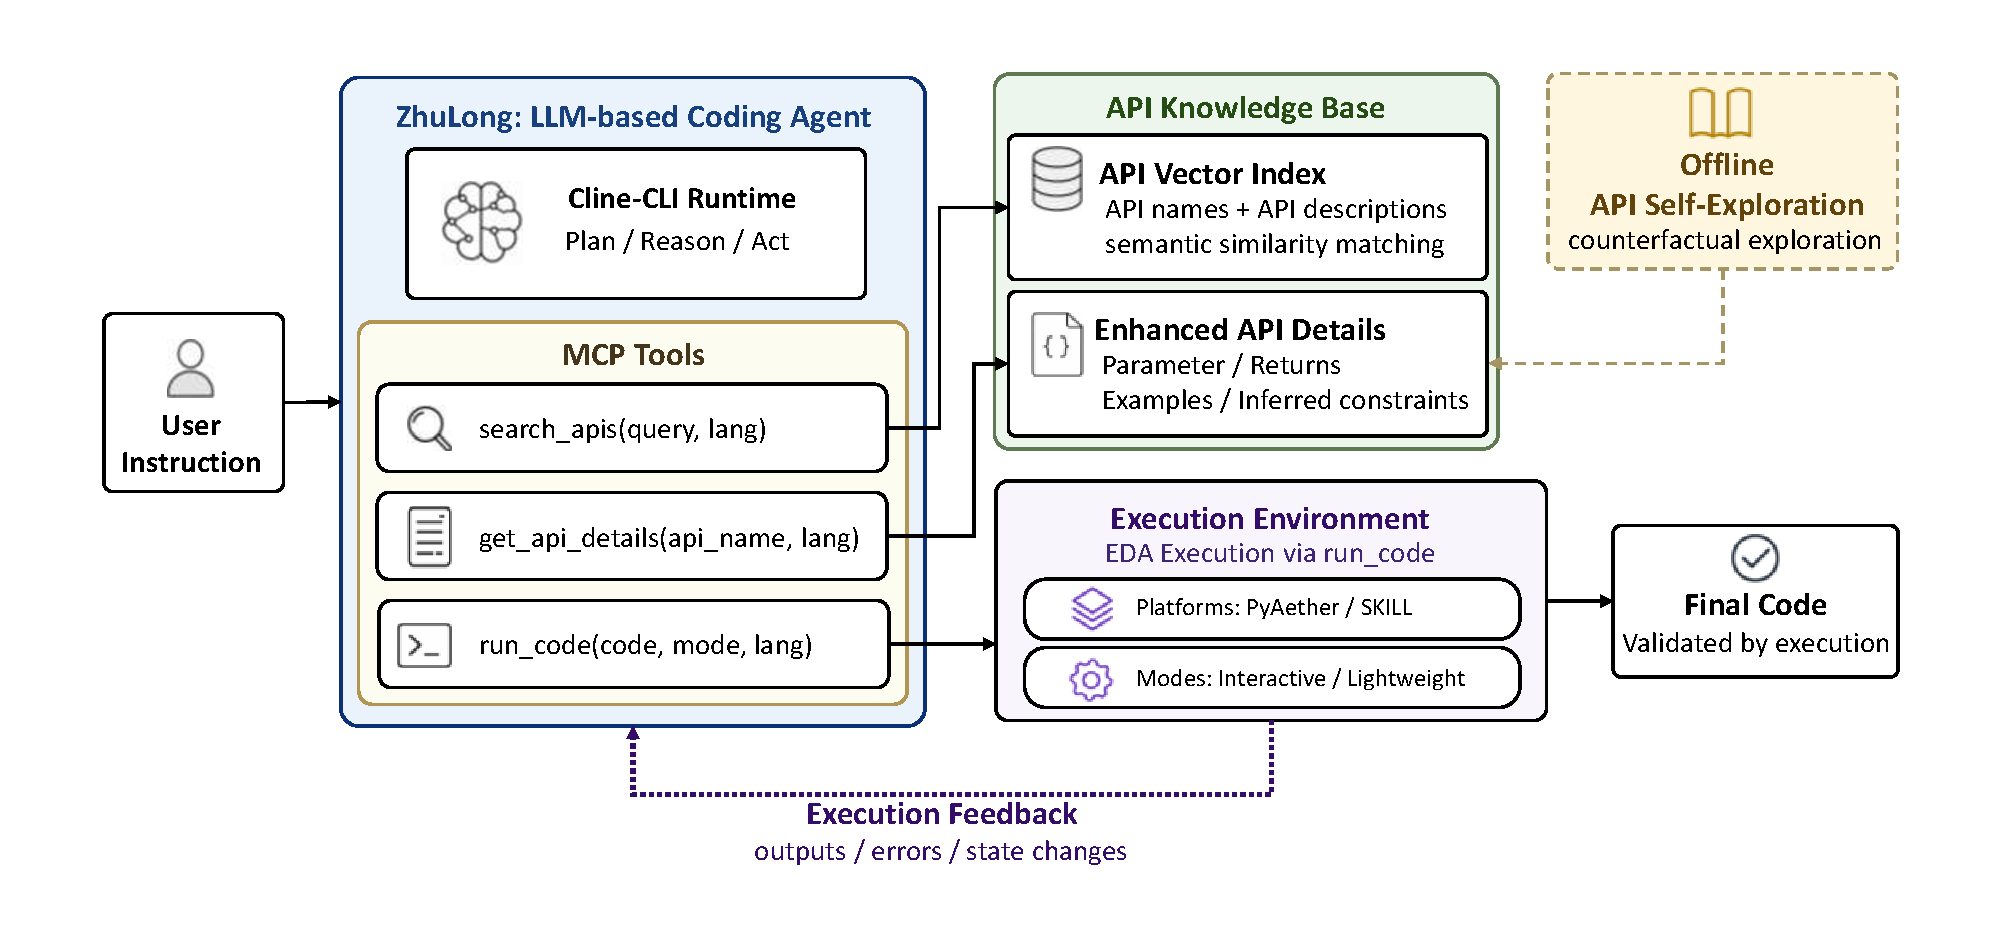
\includegraphics[width=0.9\textwidth]{figures/zhulong_arch_2.pdf}
\caption{ZhuLong system architecture. The agent interacts with API retrieval, enhanced documentation, and EDA execution via three unified MCP tools. Offline self-exploration augments the knowledge base before runtime, and execution feedback supports iterative refinement.}
% ZhuLong系统架构。智能体通过三个统一的MCP工具与API检索、增强文档和EDA执行环境交互。离线自探索在运行前增强知识库，执行反馈支持迭代优化。
\Description{Block diagram of ZhuLong's three components: the LLM agent runtime, the API knowledge base (search and retrieval), and the EDA execution sandbox. The runtime calls three MCP tools -- search_apis, get_api_details, and run_code -- with execution feedback looped back for iterative refinement; an offline self-exploration step pre-augments the knowledge base.}
\label{fig:architecture}
\end{figure*}

\subsection{Three MCP Tools}
\label{sec:mcp-tools}

ZhuLong extends three MCP tools \cite{mcp2024protocol}, each accepting a unified \texttt{lang} parameter (\texttt{pyaether}, \texttt{skill}, or \texttt{tcl}) to support all three platforms with identical agent logic:
% ZhuLong扩展了三个MCP工具 \cite{mcp2024protocol}，每个工具接受统一的\texttt{lang}参数（\texttt{pyaether}或\texttt{skill}），以相同智能体逻辑支持两个平台：

\begin{itemize}
    \item \texttt{search\_apis(query, lang)} retrieves relevant APIs via semantic and keyword-based search. We index APIs by name and description using BGE-M3 embeddings \cite{bge2024} with FAISS \cite{douze2024faiss} for efficient similarity search, returning the top-$K$ results ($K=5$ by default) with confidence scores and descriptions.
    % \texttt{search\_apis(query, lang)}通过语义和关键词检索相关API。我们使用BGE-M3嵌入 \cite{bge2024}对API名称和描述建索引，FAISS \cite{faiss2017}支持高效相似度搜索，返回top-$K$结果（默认$K=5$），附带置信度分数和描述。
    
    \item \texttt{get\_api\_details(api\_name, lang)} fetches comprehensive documentation for a specified API, including parameter types, return values, and examples. The returned documentation is augmented by the offline API self-exploration mechanism (Section~\ref{sec:selfdoc}) when available, enriching incomplete specifications with constraints and usage patterns discovered via sandbox exploration.
    % \texttt{get\_api\_details(api\_name, lang)}获取指定API的完整文档，包括参数类型、返回值和示例。当可用时，返回的文档由离线API自探索机制（第~\ref{sec:selfdoc}节）增强，补充通过沙盒探索发现的约束和使用模式。
    
    \item \texttt{run\_code(code, mode, lang)} executes the generated code in the EDA environment. It supports two modes: (1) \textbf{lightweight}—runs in a sandboxed environment without a GUI session (standalone PythonE for PyAether, or SKILL in batch mode for Virtuoso), capturing outputs, errors, and state changes for iterative refinement; (2) \textbf{interactive}—runs inside an open EDA session via the agent-EDA bridge (socket communication), enabling operations on unsaved layouts and schematics.
    % \texttt{run\_code(code, mode, lang)}在EDA环境中执行生成的代码。支持两种模式：（1）\textbf{轻量模式}——在沙盒化环境中运行，无需GUI会话（PyAether使用独立PythonE环境，Virtuoso使用SKILL批处理模式），捕获输出、错误和状态变化供迭代优化使用；（2）\textbf{交互模式}——通过agent-EDA桥接（socket通信）在已打开的EDA会话内运行，支持操作未保存的版图和原理图。
\end{itemize}

\subsection{Agent Workflow}
\label{sec:agent-workflow}

The agent iteratively refines its output through execution feedback \cite{cline2024cline}. A typical trajectory begins with reasoning over the user instruction, followed by API retrieval via \texttt{search\_apis} when needed. Candidate APIs are then inspected via \texttt{get\_api\_details}, and code is generated accordingly. The agent executes the code via \texttt{run\_code}, observes the result, and re-plans—revising the code, retrieving alternative APIs, or terminating. This loop continues until success or the agent determines further attempts are unlikely to succeed. The agent is not constrained to a fixed sequence; it may skip retrieval when it already knows the required API, or conduct multiple rounds of retrieval when initial results lack confidence.
% 智能体通过执行反馈迭代优化其输出 \cite{cline2024cline}。典型轨迹始于对用户指令的推理，需要时通过\texttt{search\_apis}检索API，然后通过\texttt{get\_api\_details}查阅候选API的文档，据此生成代码。智能体通过\texttt{run\_code}执行代码、观察结果并重规划——修改代码、检索替代API或终止。此循环持续至成功或智能体判断继续尝试不太可能成功。智能体不受固定序列约束——已知所需API时可跳过检索，初始结果置信度不足时可进行多轮检索。

\subsection{Offline API Self-Exploration (Complementary)}
\label{sec:selfdoc}

EDA API documentation is often incomplete, omitting parameter constraints, return structures, and error conditions. Prior work addresses these gaps through retrieval-based augmentation \cite{pu2024rag} or static knowledge graphs \cite{liu2025layoutcopilot}---both of which rely on what is already documented. As the theoretical framing of Section~\ref{sec:grounding-theory} makes precise, such mechanisms enrich only the L1--L3 facts the observation channel can return; they are therefore complementary to---and bounded by---the observation of L4 that requires acting on the live design. We accordingly position self-exploration as an efficiency and robustness mechanism, not as the primary accuracy driver.
% EDA工具的API文档往往不完整，省略参数约束、返回结构和错误条件。已有工作通过检索增强或静态知识图谱弥补文档缺口，但两者都依赖已有文档。
% 正如第~\ref{sec:grounding-theory}节的理论框架所指出的，这类机制只能丰富观测通道可返回的L1–L3事实；
% 因此它们相对"通过作用于实时设计来观测L4"是互补且有界的。我们将自探索定位为效率与鲁棒性机制，而非精度主驱动。

ZhuLong instead \textbf{proactively discovers} API behaviors through offline counterfactual experimentation in the sandbox. For each target API, the exploration agent reads available documentation, identifies gaps---e.g., unspecified parameter ranges, undocumented return fields, or ambiguous error semantics---and generates targeted test scripts to probe them. It executes these scripts via \texttt{run\_code}, observes outcomes, and iteratively refines a behavioral model of the API capturing parameter constraints, return structures, error conditions, and side effects. The exploration agent autonomously decides what to test next and when to stop, based on its current confidence. This offline process runs once per API; the enriched documentation is stored in the knowledge base and served at runtime via \texttt{get\_api\_details}, incurring no runtime overhead.
% ZhuLong转而通过沙盒中的离线反事实实验主动发现API行为。对每个目标API，探索智能体阅读现有文档、识别缺口、生成针对性测试脚本，通过run_code执行并观察结果，迭代细化API行为模型。探索智能体自主决定测试内容与停止时机。该离线过程每个API运行一次，增强文档存入知识库，运行时通过get_api_details提供，无额外开销。

\textbf{Implementation and cost.} The exploration agent targets the union of (i) APIs referenced by EDA-Eval-PyAether tasks and (ii) APIs whose official documentation omits at least one of parameter ranges, return types and structures, or error conditions. Each API is assigned a confidence score that accumulates the information gain of each probe; exploration terminates when the score exceeds threshold $\tau$, when two consecutive rounds contribute no new discriminated constraint, or when a per-API execution budget $M$ is exhausted. Generated test scripts are gated by EDA domain experts before execution to filter destructive operations, and discovered constraints are sanity-checked against vendor documentation where available. Exploration is a one-time offline cost per API (Table~\ref{tab:selfdoc-cost}).
% 实现与成本。探索以评测任务引用的API和官方文档缺失关键信息的API的并集为目标。每个API维护置信度分数，按每次探测的信息增益累积；当分数超过阈值、连续两轮无新增可判别约束、或单API执行预算耗尽时停止。生成的测试脚本在执行前经专家把关过滤破坏性操作。探索为每个API一次性的离线成本。

\begin{table}[htbp]
\centering
\caption{Self-exploration scale and cost (one-time, offline)}
\label{tab:selfdoc-cost}
\begin{tabular}{lc}
\toprule
\textbf{Item} & \textbf{Value} \\
\midrule
APIs targeted & [TBD] \\
APIs with $\geq 1$ discovered constraint & [TBD] \\
Average experiments per API & [TBD] \\
Average wall-clock per API (s) & [TBD] \\
Total offline wall-clock (h) & [TBD] \\
Human-reviewed test scripts & [TBD] \\
\bottomrule
\end{tabular}
\end{table}
% 表：自探索规模与成本（一次性、离线）。
% Theory precedes the benchmark and the measurements: every prediction in
% Section~\ref{sec:prediction} and every research question in Section~\ref{sec:exp-setup}
% is derived from the framework in Section~\ref{sec:grounding-theory}, rather than the
% framework being offered as an explanation after the results are known.
\section{Theoretical Grounding: The Grounding Gap}
\label{sec:grounding-theory}

Our empirical results show that the execution loop is decisive---adding sandbox execution to retrieval yields +[TBD]~pp, while removing either execution ($-[TBD]$~pp) or retrieval ($-3.2$~pp) reduces accuracy---whereas offline self-exploration yields only a modest complementary gain (+[TBD]~pp). This section explains \emph{why} this is not an accident of our implementation but a structural property of EDA scripting. We condense the \emph{grounding gap} framework: EDA scripting correctness is a \emph{situated} property that cannot be guaranteed from offline knowledge, and execution is the only channel that observes the current design state. The gap is bounded by observation fidelity, not model scale.

% 我们的实证结果表明执行闭环是决定性的（在检索之上加入沙盒执行带来+[TBD]个百分点，而移除执行或检索都会使准确率坍塌），
% 而离线自探索只带来有限的互补增益（+[TBD]个百分点）。本节解释为什么这不是实现的偶然，而是EDA脚本编写的结构性属性。
% 我们浓缩"落地鸿沟"框架：EDA脚本正确性是一个情境化属性，无法从离线知识保证，执行是观测当前设计状态的唯一通道。
% 该鸿沟受观测保真度约束，而非模型规模。

\subsection{A Four-Level Hierarchy of Information}
\label{sec:four-levels}

To make precise what can be learned offline versus what must be observed online, we distinguish four levels of information (Table~\ref{tab:four-levels}). The distinction applies to any agent whose knowledge is fixed by offline learning before deployment:
\begin{itemize}
\item \textbf{L1--Syntactic Correctness}: well-formedness of symbols according to formal rules. Captured by formal grammars and the syntactic capacities of modern LLMs.
\item \textbf{L2--Physical Plausibility}: what is physically plausible or generally expected---objects do not pass through walls, water flows downhill. L2 captures robust statistical patterns of the world, not logical certainties; these regularities are general and acquirable offline, constituting the agent's \emph{prior} over how the world typically behaves.
\item \textbf{L3--Historical Factuality}: what has actually occurred or is documented as fact. L3 concerns actual rather than merely possible states of affairs. Like L1 and L2 it can be acquired offline, but it is \emph{past-oriented}: it describes what was true as of the training cutoff, with no connection to what is true \emph{now}.
\item \textbf{L4--Situated Truthfulness}: what is true \emph{right now}, in this specific environment. Three characteristics define it: \emph{indexicality}---truth depends on context and changes over time; \emph{non-guaranteeability from offline data}---no offline dataset can \emph{guarantee} the current state, though it may induce strong priors; and \emph{real-time commitment}---L4 must be acquired continuously and acted upon promptly.
\end{itemize}

% 为了精确区分什么可以离线学习、什么必须在线观测，我们区分四个信息层次（表~\ref{tab:four-levels}）：
% L1语法正确性、L2物理合理性、L3历史事实性、L4情境真实性。前三层可离线获取，构成智能体关于世界通常如何运作的先验；
% L4由三个特征定义：指示性（真值依赖语境并随时间变化）、无法由离线数据保证（但可诱导强先验）、实时承诺（须持续获取并迅速行动）。

Two clarifications matter. First, L4 is not a semantic category of propositions; it is a \emph{grounding requirement} imposed by indexical reference---the same proposition may be L3 at one moment and L4 at another, depending on whether it refers to a past fact or a current state. Second, the four levels are not a taxonomy of all knowledge: they separate what can be \emph{known in advance} from what must be \emph{observed now}. L4 is whatever must be \emph{read} from the environment rather than \emph{recalled} from memory.

% 两点澄清：第一，L4不是命题的语义类别，而是指示性所指强加的\emph{落地要求}——同一命题在不同时刻可能属于L3或L4。
% 第二，四层区分不是知识的分类法，它区分"可预先知道"与"必须此刻观测"；L4是必须从环境中\emph{读取}而非从记忆中\emph{回忆}的东西。

\begin{table*}[htbp]
\centering
\caption{The four levels of information}
\label{tab:four-levels}
\begin{tabular}{clp{5.2cm}c}
\toprule
\textbf{Level} & \textbf{Name} & \textbf{Core Question} & \textbf{Learnable Offline?} \\
\midrule
L1 & Syntactic Correctness & Is this string well-formed? & Yes \\
L2 & Physical Plausibility & Could this event happen? & Yes \\
L3 & Historical Factuality & Did this event happen? & Yes \\
L4 & Situated Truthfulness & Is this true \emph{right now}? & \textbf{No} \\
\bottomrule
\end{tabular}
\end{table*}
% 表：四个信息层次。"能否离线学习"一列是操作性的判据：L1–L3 可以，L4 不可以。

For EDA scripting, the situated state is the live design database: which cell and view are selected, and what the layout or schematic contains at this moment. Situated states are not limited to the physical world---they include digital and informational states generally, and the user's current intent---so a clarification obtained from the user is an L4 observation as well.

% 对EDA脚本编写而言，情境状态就是实时的设计数据库：当前选中哪个cell和view、此刻版图或原理图中有什么。
% 情境状态不限于物理世界——它包括数字与信息状态，也包括用户的当前意图——因此从用户处获得的澄清同样是一次L4观测。

The correctness criterion we adopt---that generated code executes without error and all assertions over the mutated design pass---is an L4 property. A script that is well-formed (L1), plausible (L2), and invokes documented functions (L3) can nonetheless violate an undocumented binding contract, depend on an internal selection state, or target the wrong cell, and thus fail the test oracle. No amount of offline knowledge can resolve such failures; they must be \emph{observed} by acting on the live design and reading back the result. Four architectural consequences follow from L4's defining characteristics: a system trained offline and deployed frozen has no observation modules, no persistent situated state, no execution interface, and no real-time feedback loop. Every failure we analyze in Section~\ref{sec:error-analysis} traces to one or more of these.

% 我们采用的正确性判据——生成代码无错误执行且针对被修改设计的所有断言通过——是一个L4属性。
% 一个语法正确（L1）、合理（L2）、调用已文档化函数（L3）的脚本，仍可能违反未文档化的绑定契约、
% 依赖内部选中状态或定位到错误单元而失败。离线知识无法解决这类失败；它们只能通过作用于实时设计并读回结果来观测。
% 由L4的定义性特征推出四个架构性后果：离线训练并冻结部署的系统没有观测模块、没有持久情境状态、
% 没有执行接口、没有实时反馈环路。第~\ref{sec:error-analysis}节分析的每个失败都可追溯到其中之一。

\subsection{A Bayesian Formalization of the Grounding Gap}
\label{sec:bayesian}

We cast grounding as decision-making under partial observability, mirroring POMDPs and Bayesian filtering \cite{kaelbling1998planning, thrun2005probabilistic}; the formulation below is diagnostic rather than algorithmic---it is not a blueprint for tractable inference in high-dimensional state spaces, but a normative standard that makes precise \emph{what} is missing: the observation likelihood $\Omega$ and the recursive update $\Phi$.

% 我们把落地建模为部分可观测下的决策，类比POMDP与贝叶斯滤波；以下形式化是诊断性而非算法性的——
% 它不是高维状态空间中可处理推理的蓝图，而是一个规范性标准，精确指出\emph{什么}是缺失的：观测似然Ω与递归更新Φ。

Let $\Theta$ denote the space of L4 states (the live EDA design database), $o_t$ a runtime observation, $a_t$ a generated code action, and $\mathcal{K}$ the offline knowledge encoded in the LLM's frozen parameters (L1--L3). The agent maintains a belief over the current L4 state:
\begin{equation}
b_t(\theta) \triangleq p(\theta_t \mid o_{1:t},\, a_{1:t-1},\, \mathcal{K}),
\end{equation}
updated recursively by Bayes' rule:
\begin{equation}
b_t(\theta) \propto p(o_t \mid \theta_t)\, \int_{\Theta} p(\theta_t \mid \theta_{t-1}, a_{t-1})\, b_{t-1}(\theta_{t-1})\, d\theta_{t-1},
\end{equation}
where $p(o_t \mid \theta_t)$ is the \emph{observation likelihood} $\Omega$, implemented by the Harness's observation modules (Section~\ref{sec:zhuLong-harness}), and $p(\theta_t \mid \theta_{t-1}, a_{t-1})$ is the \emph{transition model} $\mathcal{T}$ supplied by the LLM's prior over how EDA operations transform the design. Actions are chosen by minimizing expected cost:
\begin{equation}
a_t^* = \arg\min_{a \in \mathcal{A}}\; \mathbb{E}_{\theta_t \sim b_t}\!\big[\mathcal{C}(\theta_t, a, G) + \gamma\, V(b_{t+1})\big],
\end{equation}
where $\mathcal{C}$ encodes the task assertions and $\gamma$ a discount factor.

% 令$\Theta$为L4状态空间（在线EDA设计数据库），$o_t$为运行时观测，$a_t$为生成的代码动作，
% $\mathcal{K}$为编码在LLM冻结参数中的离线知识（L1–L3）。智能体维护关于当前L4状态的信念$b_t(\theta)$，
% 通过贝叶斯法则递归更新。其中观测似然$\Omega$由框架的观测模块实现（第~\ref{sec:zhuLong-harness}节），
% $\mathcal{T}$为LLM先验提供的转移模型。行动通过最小化期望代价选择。

The \emph{grounding gap} is the divergence between the posterior achievable with runtime observations and the posterior from the offline prior alone:
\begin{equation}
D_{\text{grounding}}(t) \triangleq D_{\mathrm{KL}}\!\left(p(\cdot \mid o_{1:t},\, \mathcal{K},\, \text{env}) \;\middle\|\; p_{\mathcal{K}}(\cdot \mid o_{1:t})\right).
\end{equation}
This divergence is bounded by the fidelity of the observation channel, not by the capacity of the model. If $I(\Theta_t; O_t \mid \mathcal{K}) = 0$---that is, the observation channel is silent about the state---no improvement in the prior can recover the current state. Scaling $\mathcal{K}$ improves L1--L3, but it cannot reduce the gap below the floor imposed by $\Omega$.

% 落地鸿沟是有运行时观测的后验与仅靠离线先验的后验之间的散度，受观测通道保真度约束而非模型容量约束。
% 若I(Θ;O|K)=0（观测通道对状态沉默），任何先验改进都无法恢复当前状态。
% 扩大K只改善L1–L3，无法突破Ω施加的下界。

The source of the gap is causal, not statistical. Parameters are fixed before deployment; facts that come into existence after the training cutoff, or states that depend on unrepeatable circumstances, cannot be present in them by definition. The environment at time $t$ is not a function of the training corpus, and offline data and scaling affect only the prior, never the availability of runtime observation.

% 鸿沟的来源是因果性的，而非统计性的：参数在部署前固定，训练截止后产生的事实、
% 或依赖不可重复情境的状态，按定义不可能存在于参数中。t时刻的环境不是训练语料的函数；
% 离线数据与规模扩展只影响先验，不影响运行时观测的可得性。

This separates grounding from learning-based adaptation. Fine-tuning and meta-learning are capabilities acquired during \emph{training}: they improve the \emph{prior} over L1--L3 distributions. Grounding occurs during \emph{deployment} and requires the likelihood and a posterior update from observing $o_t$. A better prior does not eliminate the need for observation; the two are complementary---one offline, one online; one about knowledge, one about belief.

% 这把落地与基于学习的适应区分开：微调与元学习是\emph{训练}期获得的能力，改善的是关于L1–L3分布的先验；
% 落地发生在\emph{部署}期，需要似然与基于观测$o_t$的后验更新。更好的先验并不能消除对观测的需要；
% 两者互补——一个离线、一个在线；一个关乎知识、一个关乎信念。

\subsection{ZhuLong as an Instance of the Agent Harness}
\label{sec:zhuLong-harness}

The formulation maps onto ZhuLong's architecture. The frozen LLM supplies the prior $\mathcal{K}$ (L1--L3), the transition model $\mathcal{T}$, and an approximation to the policy $\Pi$. The Harness supplies what the LLM lacks---observation, belief update, and execution---and ZhuLong's three MCP tools instantiate it: \texttt{search\_apis} and \texttt{get\_api\_details} are the \emph{observation modules} $\Omega$, reading documented API facts out of the environment; \texttt{run\_code} is the \emph{effector} that acts on the live design database, whose resulting state is transduced into textual observations (stdout, errors, assertion outcomes). The re-planning loop (Section~\ref{sec:agent-workflow}) implements the belief update $\Phi$: each observation $o_t$ revises the agent's belief about which API contracts and compositions actually hold. The closed loop $b_t \to a_t \to o_{t+1} \to b_{t+1}$ is what turns one-shot generation into grounded search; grounding is a property of the coupled system, not of the model alone.

% 该形式化直接映射到ZhuLong架构。冻结的LLM提供先验$\mathcal{K}$（L1–L3）、转移模型$\mathcal{T}$以及策略$\Pi$的近似。
% 框架提供LLM所缺乏的观测、信念更新与执行，ZhuLong的三个MCP工具将其实例化：
% \texttt{search\_apis}与\texttt{get\_api\_details}是\emph{观测模块}$\Omega$，从环境中读取已文档化的API事实；
% \texttt{run\_code}是\emph{执行器}，作用于实时设计数据库，其结果状态被转换为文本观测（stdout、错误、断言结果）。
% 重规划循环（第~\ref{sec:agent-workflow}节）实现信念更新$\Phi$：每次观测$o_t$修正智能体关于哪些API契约与组合确实成立的信念。
% 闭环 $b_t \to a_t \to o_{t+1} \to b_{t+1}$ 把一次性生成变为接地搜索；落地是耦合系统的属性，而非模型单独的属性。

\subsection{Design Principles}
\label{sec:prediction}

The formalization yields three architectural principles: \emph{freeze} $\mathcal{K}$, \emph{maximize} the fidelity of $\Omega$, and \emph{run} $\Phi$ \emph{continuously}.

\textbf{Decouple knowledge from belief.} Knowledge $\mathcal{K}$ is the static L1--L3 prior encoded in the LLM's parameters---general and context-free; belief $b_t(\theta)$ is the dynamic posterior maintained by the Harness---specific and context-dependent. Updating $\mathcal{K}$ with the limited observations available during deployment is inefficient and risks catastrophic forgetting, and even a prior enriched offline cannot substitute for observation; freezing $\mathcal{K}$ and absorbing adaptation in $b_t$ yields stability and flexibility at once.

\textbf{Optimize observation over the prior.} The gap is bounded by the fidelity of the likelihood $\Omega$, not by the expressiveness of the prior: $D_{\text{grounding}}(t)$ is bounded by $\|\tilde{p} - p_{\text{real}}\|$, a bound independent of model scale. Investment in observation---retrieval and documentation quality, execution read-back, state estimation---therefore has a direct and bounded effect, whereas investment in model scale has diminishing returns once the prior is sufficiently rich, because it cannot push the gap below the floor imposed by observation.

\textbf{Design for continuous belief updating.} $\Phi$ operates online: every observation yields a recursive update $b_t \mapsto b_{t+1}$. Two implications follow. First, $\Phi$'s update rate must exceed the timescale of L4 dynamics, otherwise $b_t$ goes stale. Second, $b_t$ must be a structured representation that captures uncertainty and history, so that the agent can recover from unexpected changes. In the ICL-type autonomous agent of Section~\ref{sec:system}, $\Phi$ has no explicit posterior: it is approximated by in-context learning, since each returned observation is appended and conditions the next decision, while the agent decides for itself when the result is good enough to submit. Because such an agent is autonomous, the quantity to bound is not a count of ``rounds''---it has none---but how much evidence its belief state may ever accumulate: a graded budget on the executions it may observe, or a read-back that lags the action it reports.

% 形式化给出三条架构原则：冻结$\mathcal{K}$、最大化$\Omega$保真度、持续运行$\Phi$。
% （一）解耦知识与信念：$\mathcal{K}$是LLM参数中编码的静态L1–L3先验，$b_t$是框架维护的动态后验；
% 用部署期有限的观测去更新$\mathcal{K}$既低效又有灾难性遗忘风险，且离线增强的先验也无法替代观测。
% （二）优先优化观测而非先验：鸿沟受似然$\Omega$保真度约束（上界$\|\tilde{p}-p_{\text{real}}\|$与模型规模无关）；
% 观测投入有直接有界的效果，模型规模投入在先验足够丰富后收益递减。
% （三）为持续信念更新而设计：$\Phi$的更新率必须超过L4动态的时间尺度，且$b_t$须是捕获不确定性与历史的结构化表征。

These principles \emph{account for} our ablation findings rather than merely restating them. Removing the observation channel (``ZhuLong w/o Sandbox'') leaves $b_t$ uninformative: with no $\Omega$, L4 violations such as hidden type contracts and internal selection state (Section~\ref{sec:error-analysis}) are unobservable by construction, and Pass@1 drops by [TBD]~pp. A retrieval-only system (RAG, 70.3\%) improves the L1--L3 prior but still cannot observe L4, so its ceiling is bounded by what offline knowledge can guarantee. The offline API self-exploration mechanism (Section~\ref{sec:selfdoc}) likewise improves only the L1--L3 facts the harness can supply---it enriches documentation with discovered constraints---and is therefore \emph{complementary and bounded}: it reduces uncertainty about contracts but cannot replace observation of the current state, which is why its contribution (+[TBD]~pp) is dwarfed by that of the observation channel.

% 这些原则\emph{解释}而非仅仅复述了消融结果：移除观测通道使$b_t$失去信息，L4违规在构造上不可观测，
% Pass@1下降[TBD]个百分点；仅检索系统（RAG）改善L1–L3先验但无法观测L4，其上界受离线知识所能保证的范围约束；
% 离线API自探索改善的同样是\emph{先验}，因而是互补且有界的。

Three diagnostic questions follow for any candidate system: (1)~does it implement $\Omega$ with sufficient fidelity to track L4 dynamics? (2)~does it maintain $b_t$ as a structured state, updated through $\Phi$ after each observation? (3)~does it approximate $\Pi$ from offline knowledge and execute $a_t$ through a causal interface? Section~\ref{sec:experiments} answers them for ZhuLong, on the benchmark constructed in Section~\ref{sec:benchmark}.

% 由此得到三个诊断性问题：(1) 是否以足够保真度实现$\Omega$以追踪L4动态；
% (2) 是否将$b_t$维护为经$\Phi$更新的结构化状态；(3) 是否用离线知识近似$\Pi$并通过因果接口执行$a_t$。
% 下一节针对ZhuLong回答这三点。

These principles and questions organize the evaluation into three research questions (Section~\ref{sec:exp-setup}): whether the ceiling is set by observation or by the prior (RQ1), which components are necessary and whether they are interchangeable (RQ2), and whether the structure follows from the domain class rather than from one toolchain (RQ3).
% 这些原则与诊断问题把评估组织为三个研究问题（第~\ref{sec:exp-setup}节）：
% 天花板由观测还是先验设定（RQ1）；哪些组件是必要的以及它们可否互换（RQ2）；
% 以及该结构是否源于领域类而非某个工具链（RQ3）。




\section{Benchmark Construction}
\label{sec:benchmark}

\subsection{Dataset: EDA-Scripting-Bench}

For DAC, we assemble \textbf{EDA-Scripting-Bench}, a unified cross-language benchmark spanning three EDA scripting languages---PyAether, SKILL, and Tcl---under one task schema and one execution-based protocol. Every task carries a \texttt{lang} field and language-appropriate assertions, so a single agent harness (Section~\ref{sec:agent-workflow}) can be scored uniformly across platforms. At present EDA-Scripting-Bench contains one completed slice, \textbf{EDA-Eval-PyAether} (158 PyAether tasks), with the SKILL and Tcl slices under construction. Consequently, all quantitative results in this draft are provisional and will be regenerated on the full EDA-Scripting-Bench.

\subsection{Dataset: EDA-Eval-PyAether (PyAether slice)}

To evaluate LLM-based code generation for PyAether, we constructed \textbf{EDA-Eval-PyAether}, the 158-task PyAether slice of EDA-Scripting-Bench. Tasks were collected from four sources: API references (61.4\%), documentation examples (27.2\%), internal training materials (7.6\%), and anonymized CAD practical cases (3.8\%). Each task underwent manual review by EDA domain experts.
% 为了评估基于LLM的PyAether代码生成，我们构建了\textbf{EDA-Eval-PyAether}评测集，包含158个任务。任务收集自四个来源：API参考文档（61.4\%）、官方文档示例（27.2\%）、内部培训材料（7.6\%）和脱敏的CAD实际案例（3.8\%）。每个任务均由EDA领域专家进行了人工审核。

Table~\ref{tab:scenario-distribution} shows the distribution of tasks across different EDA scenarios. Layout and Schematic operations constitute the majority (70.2\%), reflecting the core focus of PyAether usage in physical design workflows.
% 表~\ref{tab:scenario-distribution}展示了任务在不同EDA场景中的分布。Layout和Schematic操作占大多数（70.2\%），反映了PyAether在物理设计工作流中的核心使用场景。

\begin{table}[htbp]
\centering
\caption{Task distribution by scenario}
\label{tab:scenario-distribution}
\begin{tabular}{lcc}
\toprule
\textbf{Scenario} & \textbf{Tasks} & \textbf{Percentage} \\
\midrule
Layout & 64 & 40.5\% \\
Schematic & 47 & 29.7\% \\
Design Management & 24 & 15.2\% \\
Others & 23 & 14.6\% \\
\midrule
Total & 158 & 100\% \\
\bottomrule
\end{tabular}
\end{table}
% 表：按场景划分的任务分布。

\subsection{Evaluation Protocol}

Each task consists of a natural language prompt, a function signature, and assertion-based test code. A task is considered passed if the generated code executes in the PyAether sandbox without errors and all assertions pass. The primary metric is Pass@1 \cite{chen2021evaluating}:
% 每个任务包含三个部分：自然语言提示、函数签名、以及基于断言的测试代码。如果生成的代码在PyAether沙盒中无错误执行且所有断言通过，则该任务被视为通过。主要指标为Pass@1 \cite{chen2021evaluating}：

\[
\text{Pass@1} = \frac{\text{\# tasks with all assertions passed}}{\text{Total tasks}} \times 100\%
\]
% \[
% \text{Pass@1} = \frac{\text{所有断言均通过的任务数}}{\text{总任务数}} \times 100\%
% \]
\section{Experiments}
\label{sec:experiments}

\subsection{Experimental Setup}
\label{sec:exp-setup}

\subsubsection{Research Questions}

The framework of Section~\ref{sec:grounding-theory} makes three testable claims: that the grounding gap is bounded by observation fidelity rather than by the prior; that bridging it requires a runtime architecture supplying observation, belief update and execution; and that this follows from the domain's structure rather than from one toolchain. We ask one research question per claim.
% 第~\ref{sec:grounding-theory}节的框架给出三条可检验主张：落地鸿沟受观测保真度而非先验约束；
% 弥合它需要一个同时提供观测、信念更新与执行的运行时架构；这一点源于领域结构而非某个工具链。
% 我们针对每条主张提出一个研究问题。

\begin{itemize}
\item \textbf{RQ1 (Ceiling: observation or prior?).} Is the achievable accuracy bounded by the fidelity of the observation channel $\Omega$, or by the strength of the frozen prior $\mathcal{K}$? We answer from both sides: the observation-fidelity ladders (S1) vary $\Omega$ with the LLM fixed, and the prior-axis contrast (S3) varies $\mathcal{K}$ with the harness fixed.
\item \textbf{RQ2 (Which components are necessary, and are they interchangeable?).} Does bridging the gap require observation, execution through a causal interface, and continuous belief update---and can one of the three substitute for another? S2 varies the effector's presence and the belief-update budget.
\item \textbf{RQ3 (Domain class or toolchain?).} Does the same structure reproduce on a structurally different toolchain? The protocol of S1--S2 is re-run on the SKILL and Tcl slices of \textbf{EDA-Scripting-Bench}, so the comparison is made \emph{within} one benchmark rather than across separate artifacts.
\end{itemize}
% RQ1（天花板：观测还是先验？）可达准确率受观测通道$\Omega$的保真度约束，还是受冻结先验$\mathcal{K}$的强度约束？
% 我们从两侧回答：保真度阶梯（S1）固定LLM改变$\Omega$；先验轴对照（S3）固定框架改变$\mathcal{K}$。
% RQ2（哪些组件是必要的？它们可互换吗？）弥合鸿沟是否同时需要观测、经由因果接口的执行、以及持续的信念更新？
% 三者能否相互替代？S2改变执行器是否在场与信念更新预算。
% RQ3（领域类还是工具链？）同一结构能否在结构不同的工具链上复现？
% S1–S2的协议在EDA-Scripting-Bench的SKILL与Tcl切片上重跑，因此比较发生在同一评测集内部，而非跨不同工件。

RQ1 and RQ2 test the framework's structural claims; RQ3 tests whether they follow from the domain's structure rather than from one toolchain. Because RQ1's two arms sit in different studies, we read them against each other rather than in isolation.
% RQ1与RQ2检验框架的结构性主张；RQ3检验这些主张是否源于领域结构而非某个工具链。
% 由于RQ1的两个臂分布在不同研究中，我们将其相互对照而非单独解读。

\subsubsection{Benchmark and Evaluation Protocol}

We evaluate ZhuLong on \textbf{EDA-Eval-PyAether}, a benchmark of 158 real-world PyAether scripting tasks. Following the evaluation protocol defined in Section~\ref{sec:benchmark}, we adopt \textbf{Pass@1} (execution success rate) as the primary metric. Each task is evaluated in a single trace: the agent may iterate \emph{within} that trace through the belief update $\Phi$ (Section~\ref{sec:agent-workflow}), but a task is never restarted across traces; the timeout is set to 2500 seconds per execution. Every tool call is additionally mediated by a file-based \texttt{PreToolUse} hook---a JSON-in/JSON-out script dispatched by Cline's hook engine from the configured hooks directory---that enforces a tool whitelist, blocks shell and code-search tools, and confines all file access to a fresh, empty working directory; on each call it allows the call, rewrites it to a harmless no-op (\texttt{overrideInput}), or rejects it with an error message (\texttt{cancel}), with MCP tool calls passing through, so neither a task's own assertions nor any project copy of a solution is reachable from the workspace. The hook is identical in every configuration reported here and is thus part of the fixed protocol rather than a variable; it is also what makes the baselines interpretable. Traces terminated by the hook are identified separately so that they are not read as capability failures. To assess statistical reliability given the modest benchmark size (158 tasks), each configuration is evaluated over five independent runs with reshuffled task orderings and fresh agent contexts, and accuracy is reported as mean $\pm$ standard deviation over those runs. Quantities aggregated over traces rather than over runs---read-back counts, activation ratios and tool-call totals---are given as single aggregates over the pooled traces, without run-level dispersion; effect sizes ($\Delta$) are computed from the mean values in the same table. The dominant sandbox-execution effect ($+[TBD]$ pp) exceeds the spread by an order of magnitude, whereas the smaller self-exploration effect ($+[TBD]$ pp) is treated as a complementary gain rather than a headline result, consistent with the theoretical account in Section~\ref{sec:grounding-theory}. All figures in this section are provisional, obtained on the PyAether-only slice, and will be regenerated on the full EDA-Scripting-Bench (Section~\ref{sec:benchmark}).
% 评测集与评估协议。我们在\textbf{EDA-Eval-PyAether}上评估ZhuLong，该评测集包含158个真实PyAether脚本任务。
% 遵循第\ref{sec:benchmark}节定义的评估协议，我们采用\textbf{Pass@1}（执行成功率）作为主要指标。
% 每个任务只在单条trace上评测：智能体可在该trace内通过信念更新$\Phi$（第\ref{sec:agent-workflow}节）反复迭代，
% 但任务绝不跨trace重启；单次执行超时设为2500秒。此外，每次工具调用都经由框架层\texttt{PreToolUse} hook 中介：
% 它执行工具白名单，并把文件读写限制在一个新建的空工作目录内，使任务的断言文件与任何项目内的参考解都不可达。
% 该 hook 在所有配置中完全一致，属于固定协议而非变量，也是基线可解释的前提。
% 因它终止的trace单独标识，以免被误读为能力不足。鉴于评测集规模有限（158题），
% 每个配置在5次独立运行上评测，每次重排任务顺序并使用全新智能体上下文；准确率以5次运行的均值$\pm$标准差报告。
% 跨trace（而非跨运行）汇总的量——回读次数、激活比例、工具调用总量——按合并后的trace给出单一汇总值，
% 不附运行间散布；效应量（$\Delta$）由同表的均值算出。

\subsubsection{Baselines and ZhuLong Variants}

To isolate the contribution of each component, we establish two baselines and three ZhuLong variants, as shown in Table~\ref{tab:configurations}. Read against the framework of Section~\ref{sec:grounding-theory}, the table's columns name the components a harness supplies: retrieval and documentation are the observation channel $\Omega$, the sandbox is the effector through which an action reaches the live design, and self-exploration is offline enrichment of the documentation that $\Omega$ can return. ZhuLong variants default to vector retrieval using a name+description index; S1 varies the fidelity of that index explicitly, and S2 adds a bound on the belief update $\Phi$, which this table does not vary.
% 基线与ZhuLong变体。按第~\ref{sec:grounding-theory}节的框架解读，表中三列就是框架所提供的三个组件：
% 检索与文档是观测通道$\Omega$，沙盒是使动作抵达实时设计的执行器，自探索则是对$\Omega$可返回文档的离线增强。
% ZhuLong变体默认使用名称+描述索引进行向量检索；S1显式改变该索引的保真度，S2则对信念更新$\Phi$加界——这是本表未涉及的组件。

These columns name components that are realized at the harness boundary rather than inside the agent. The presence of each observable capability is switched by a tool-registration toggle---a single disabled-list in the server environment spanning the four core tools \texttt{search\_apis}, \texttt{search\_apis\_by\_keyword}, \texttt{get\_api\_details} and \texttt{run\_code}: a disabled tool simply disappears from the agent's tool set, while every enabled tool keeps a byte-identical implementation across all arms. The sandbox executor is removed by unregistering \texttt{run\_code}; retrieval is removed by unregistering the three retrieval tools; the anti-leak \texttt{PreToolUse} hook stays loaded in every arm; and the self-exploration toggle swaps the enriched knowledge base rather than any runtime tool.
% 这些列命名的组件在框架边界实现，而非智能体内部。每个可观测能力的有无由一个"工具注册开关"切换——服务器环境里的单一禁用清单，覆盖核心 4 工具（search_apis / search_apis_by_keyword / get_api_details / run_code）：被禁用的工具从智能体工具集中消失，而每个启用的工具在各臂之间保持逐字一致的实现。关沙盒=取消注册 run_code；关检索=取消注册三个检索工具；反作弊 PreToolUse hook 每个臂始终装载；自探索开关替换增强知识库，而非任何运行时工具。

\begin{table}[htbp]
\centering
\caption{Configurations and their components}
\label{tab:configurations}
\begin{tabular}{lccc}
\toprule
\textbf{Configuration} & \textbf{Retrieval} & \textbf{Sandbox} & \textbf{Self-Expl.} \\
\midrule
Baseline 1 (Pure LLM) & \ding{55} & \ding{55} & \ding{55} \\
Baseline 2 (RAG) & \ding{51} & \ding{55} & \ding{55} \\
ZhuLong w/o Self-Expl. & \ding{51} & \ding{51} & \ding{55} \\
ZhuLong w/o Sandbox & \ding{51} & \ding{55} & \ding{51} \\
ZhuLong w/o Retrieval & \ding{55} & \ding{51} & \ding{51} \\
\textbf{ZhuLong} (Full) & \ding{51} & \ding{51} & \ding{51} \\
\bottomrule
\end{tabular}
\end{table}
% 表：配置及其组件。ZhuLong（完整）为完整系统，其余为消融变体。
% Self-Expl. = Self-Exploration mechanism.

\subsubsection{LLM Backbones}

All main experiments use DeepSeek-V4-Pro as the primary backbone. To understand the impact of different LLMs, we additionally evaluate GLM-5.2, DeepSeek-V4-Flash, Kimi-K2.6, and Doubao-Seed-2.0-Pro.
% LLM主干。所有主要实验使用DeepSeek-V4-Pro作为主要主干。为了解不同LLM的影响，我们还评估了GLM-5.2、DeepSeek-V4-Flash、Kimi-K2.6和Doubao-Seed-2.0-Pro。

\subsection{Results and Ablations}
\label{sec:exp-results}

The framework of Section~\ref{sec:grounding-theory} fixes what each study must vary. Table~\ref{tab:main-ablation} gives the progressive build-up and the component ablation as an overview; the studies below then change one component at a time, with the LLM frozen unless stated otherwise.
% 结果与消融。第~\ref{sec:grounding-theory}节的框架规定了每项研究必须改变什么。
% 表~\ref{tab:main-ablation}给出渐进构建与组件消融作为总览；以下研究每次只改变一个组件，除特别说明外固定LLM。

\begin{table}[htbp]
\centering
\caption{Ablation study results}
\label{tab:main-ablation}
\begin{tabular}{lcc}
\toprule
\textbf{Configuration} & \textbf{Pass@1 (\%)} & \textbf{$\Delta$} \\
\midrule
\multicolumn{3}{l}{\textit{Progressive build-up (vs. previous row)}} \\
Baseline 1: Pure LLM & 11.4 $\pm$ [TBD] & — \\
Baseline 2: RAG & 70.3 $\pm$ [TBD] & +58.9 pp \\
ZhuLong w/o Self-Expl. & [TBD] $\pm$ [TBD] & +[TBD] pp \\
\textbf{ZhuLong} (Full) & \textbf{84.8 $\pm$ [TBD]} & \textbf{+[TBD] pp} \\
\midrule
\multicolumn{3}{l}{\textit{Component ablation (vs. ZhuLong Full)}} \\
ZhuLong w/o Self-Expl. & [TBD] $\pm$ [TBD] & -[TBD] pp \\
ZhuLong w/o Sandbox & [TBD] $\pm$ [TBD] & -[TBD] pp \\
ZhuLong w/o Retrieval & 81.6 $\pm$ [TBD] & -3.2 pp \\
\bottomrule
\end{tabular}
\end{table}
% 表：渐进构建与组件消融研究。上块为渐进构建，"Gain"表示
% 相对于前一行的增量；下块为组件消融，"Drop"均表示相对于
% ZhuLong完整系统（加粗行）的减量。

\subsubsection{S1: Observation fidelity (RQ1)}
\label{sec:omega-fidelity}

Principle 2 predicts that with the model fixed, accuracy is bounded by the fidelity of the observation channel $\Omega$. We vary $\Omega$ along the two axes through which it receives information, holding the LLM fixed in both.

\textbf{Documentation axis.} Table~\ref{tab:omega} holds the agent loop, the effector and the LLM fixed, and changes only how faithfully the environment's API facts are exposed: no observation at all; a low-fidelity index built from API names alone; a high-fidelity index that adds descriptions, BM25 term matching, abbreviation expansion and synonym redirect; and the high-fidelity index further enriched by offline self-exploration (Section~\ref{sec:selfdoc}).
% 文档轴。表~\ref{tab:omega}固定智能体循环、执行器与LLM，只改变环境的API事实被暴露的保真度：
% 无观测；仅由API名称构建的低保真索引；加入描述、BM25词项匹配、缩写展开与同义词重定向的高保真索引；
% 以及在高保真索引上再经离线自探索增强（第~\ref{sec:selfdoc}节）。

\begin{table}[htbp]
\centering
\caption{Observation fidelity along the documentation axis (LLM, effector and loop fixed)}
\label{tab:omega}
\footnotesize
\begin{tabular}{@{}llc@{}}
\toprule
\textbf{Rung} & \textbf{Configuration} & \textbf{Pass@1 (\%)} \\
\midrule
(N) No observation & Baseline 1 (Pure LLM) & 11.4 $\pm$ [TBD] \\
(L) Low fidelity & name-only index & [TBD] $\pm$ [TBD] \\
(H) High fidelity & \shortstack[l]{+ description, BM25,\\ abbreviations, synonyms} & [TBD] $\pm$ [TBD] \\
\shortstack[l]{(H+E) High fidelity,\\ self-explored} & \textbf{ZhuLong} (Full) & 84.8 $\pm$ [TBD] \\
\bottomrule
\end{tabular}
\end{table}
% 表：Ω保真度阶梯（文档轴）。固定LLM、执行器与循环，仅改变API事实暴露的保真度。
% 注：ICML 稿中同一阶梯报告为 (N)=0.0%、(L)=59.5%、(H)=87.3%——与本表的 (N)/(H+E) 口径不同，
% 需先统一配置定义与评测协议，再决定引用哪一组数值。

\textbf{Read-back axis.} The second axis is how much of the live state execution returns. Section~\ref{sec:bayesian} predicts that accuracy tracks this fidelity with the LLM held fixed; we therefore compare three closed-loop variants that differ only here: (N) \emph{no observation}---the agent predicts from the prior alone; (B) \emph{binary feedback}---\texttt{run\_code} reports only pass/fail; and (F) \emph{full observation}---stdout, exception traces, per-assertion outcomes, and queried state are returned (the default). We expect a monotone gain N $<$ B $<$ F, with the N-to-F gap interpreting the grounding gap in practice.
% 回读轴。第二条轴是执行返回多少实时状态信息。第~\ref{sec:bayesian}节预测固定LLM时准确率随该保真度变化，
% 因此我们比较仅在此处不同的三个闭环变体：(N) 无观测、(B) 二值反馈、(F) 全观测。预期 N < B < F 单调增益，
% 其中 N→F 的差距即落地鸿沟的实操化。

Table~\ref{tab:ablation-harness} reports Pass@1 and the mean number of execution read-backs per variant.
% 表~\ref{tab:ablation-harness}报告各变体的 Pass@1 与平均信念更新轮数。

\begin{table}[htbp]
\centering
\caption{Observation-fidelity ablation along the read-back axis (RQ: Principle 2)}
\label{tab:ablation-harness}
\small
\begin{tabular}{@{}lcc@{}}
\toprule
\textbf{Observation channel ($\Omega$)} & \textbf{Pass@1 (\%)} & \textbf{Mean read-backs} \\
\midrule
(N) None (prior only) & [TBD] $\pm$ [TBD] & [TBD] \\
(B) Binary pass/fail & [TBD] $\pm$ [TBD] & [TBD] \\
(F) Full observation & [TBD] $\pm$ [TBD] & [TBD] \\
\bottomrule
\end{tabular}
\end{table}
% 表：回读轴上的观测保真度消融（原则2）。

\textbf{The self-exploration rung.} The top rung of Table~\ref{tab:omega} adds constraints discovered offline by counterfactual experimentation (Section~\ref{sec:selfdoc}). Per the framework this enriches only the L1--L3 facts the observation channel can return, so it should move the result less than the channel's own fidelity does. Removing it while keeping retrieval and the effector reduces Pass@1 from 84.8\% to [TBD]\%, a drop of [TBD] percentage points. In the absence of the effector the same mechanism improves Pass@1 from 70.3\% (RAG) to [TBD]\%, a gain of [TBD] percentage points---so the same prior-side enrichment is worth more when the observation channel is weaker, consistent with its being bounded by observation rather than substituting for it.
% 自探索档。表~\ref{tab:omega}的最高档加入经离线反事实实验发现的约束（第~\ref{sec:selfdoc}节）。
% 按框架，它只丰富观测通道可返回的L1–L3事实，因此其效应应小于通道自身保真度带来的效应。
% 保留检索与执行器而移除它，Pass@1从84.8\%降至[TBD]\%（-[TBD]pp）。
% 无执行器时同一机制把Pass@1从70.3\%（RAG）提升至[TBD]\%（+[TBD]pp）——
% 同一先验侧增强在观测通道更弱时价值更大，与"它被观测所界定而非替代观测"一致。

Beyond accuracy, this rung also changes efficiency. Table~\ref{tab:selfdoc-efficiency} compares tool usage with and without self-exploration. With self-exploration enabled the agent produces more traces (243 vs. 220) because it persists longer with better documentation, yet total tool calls drop by 13.9\% and average calls per trace decrease by 22.1\%.

\begin{table}[htbp]
\centering
\caption{Overall tool usage: with vs. without self-exploration}
\label{tab:selfdoc-efficiency}
\begin{tabular}{lcc}
\toprule
\textbf{Metric} & \textbf{w/o Self-Expl.} & \textbf{ZhuLong (Full)} \\
\midrule
Traces & 220 & 243 (+10.5\%) \\
\#Calls & 6,791 & 5,845 (-13.9\%) \\
Avg/Trace & 30.9 & 24.1 (-22.1\%) \\
\midrule
Change & — & \textbf{-946 (-13.9\%)} \\
\bottomrule
\end{tabular}
\end{table}
% 表：整体工具使用情况：启用与未启用API自探索的对比。

The reduction is most pronounced in \texttt{run\_code} (27.0\%, see Table~\ref{tab:tool-breakdown}), indicating that enriched documentation reduces trial-and-error executions. Calls to \texttt{search\_apis} decrease by 12.2\%, while \texttt{get\_api\_details} increase by 9.0\%---a behavioral shift toward more thorough reading before coding.

\begin{table}[htbp]
\centering
\caption{Tool-wise call count breakdown}
\label{tab:tool-breakdown}
\begin{tabular}{lcc}
\toprule
\textbf{Tool} & \textbf{w/o Self-Expl.} & \textbf{ZhuLong (Full)} \\
\midrule
\texttt{search\_apis} & 3,203 & 2,812 (-12.2\%) \\
\texttt{get\_api\_details} & 1,151 & 1,255 (+9.0\%) \\
\texttt{run\_code} & 2,437 & 1,778 (-27.0\%) \\
\bottomrule
\end{tabular}
\end{table}
% 表：各工具调用次数明细。

\subsubsection{S2: The closed loop (RQ2)}
\label{sec:closed-loop}

Principle 3 requires two things: that actions reach the design through a causal interface, and that the belief update $\Phi$ run continuously.

\textbf{Effector: does the action reach the live design?} Removing the sandbox from the full system drops Pass@1 from 84.8\% to [TBD]\% ($-[TBD]$~pp); adding it to the RAG baseline raises it from 70.3\% to [TBD]\% ($+[TBD]$~pp). Without an effector no $a_t$ is executed against the design, so $b_t$ receives no evidence about the live state at all and the agent is reduced to a prior-only predictor. We attribute the gain to two mechanisms: execution returns concrete error messages that guide corrections, transforming one-shot generation into iterative search, and it lets the agent probe parameter combinations that documentation omits~\cite{kumar2026agentforge, jiang2024seed}.
% 执行器：动作是否抵达实时设计？从完整系统移除沙盒使Pass@1从84.8\%降至[TBD]\%（-[TBD]pp）；
% 把沙盒加入RAG基线使其从70.3\%升至[TBD]\%（+[TBD]pp）。没有执行器，$a_t$未被作用于设计，
% $b_t$得不到任何关于实时状态的证据，智能体退化为仅凭先验的预测器。

\textbf{Belief update: how much evidence may $\Phi$ accumulate?} ZhuLong is an ICL-type autonomous agent: once the task is issued it plans, queries the API knowledge base, and executes and debugs code on its own, and it is the agent---not the harness---that decides when the result is good enough to submit. We therefore do not shorten the loop or force an early submission; we bound how often the loop \emph{may execute}, which is what determines how much state evidence $b_t$ ever receives. Operationally the bound is the number of \texttt{run\_code} calls a trace is allowed: once the budget is spent, the call is denied at the tool boundary by a second, co-resident \texttt{PreToolUse} hook that counts \texttt{run\_code} calls per trace; its error carries a unique \texttt{{[PHI-BUDGET-EXHAUSTED]}} prefix because Cline's hook engine OR-merges cancellations and concatenates their reasons, which would otherwise make the anti-leak hook's denials indistinguishable from the budget hook's, and the agent keeps running under its own control until it chooses to submit. Because termination stays with the agent, we report the harness's own finish reason next to accuracy---\emph{completed} (the agent decided it was done) versus \emph{max iterations} or budget-denied---so that a tight budget cannot be mistaken for early convergence. In an agent with no explicit posterior, $\Phi$ is realized by what remains in the model's context, so Table~\ref{tab:phi-bound} additionally includes a lagged channel realized as a single-slot ($L{=}1$) buffer in the \texttt{run\_code} handler, whose read-back returns the state emitted by the previous execution---with a \texttt{reported\_call\_index} recorded so the one-step lag is auditable---leaving the agent permanently one action behind the design; the first read-back carries no state, and every other setting is unchanged. Both axes leave the LLM, the observation content and the effector untouched. Principle 3 predicts that accuracy rises with the execution budget but saturates once updates are fast enough for the design's own dynamics, since evidence obtained before the previous action is partly obsolete by the time the next action is chosen.
% 信念更新：$\Phi$可累积多少证据？ZhuLong是自主智能体：任务下达后自行规划、查询API知识库、
% 执行并调试代码，并由智能体（而非框架）决定结果何时足够好可以提交。
% 因此我们不缩短循环、也不强制提前提交，而是给"循环可执行的次数"加界——
% 这决定了$b_t$究竟能收到多少状态证据。操作上该界就是单条trace允许的\texttt{run\_code}调用次数：
% 预算耗尽后，调用在工具边界被"第二个共存的 PreToolUse hook"（按 trace 计数 run_code 调用）拒绝，并返回带唯一前缀 \texttt{{[PHI-BUDGET-EXHAUSTED]}} 的说明性错误（Cline hook 引擎对 cancel 做 OR 合并、对原因做换行拼接，无前缀就无法与反作弊 hook 的拒绝区分）；智能体仍在自主控制下继续运行，直到自行提交。
% 由于终止权仍归智能体，我们在准确率旁报告框架自身的结束原因——
% \emph{completed}（智能体自认完成）对比\emph{max iterations}或预算被拒——
% 以便紧预算不会被误读为提前收敛。对于没有显式后验的智能体，$\Phi$由上下文留存的内容实现，
% 因此表~\ref{tab:phi-bound}另含一条"滞后"通道：其回读返回的是"上一次执行"产生的状态，
% 使智能体永远落后于设计一步；首次回读不含状态，其余设置全部不变。
% 两条轴都不动LLM、观测内容与执行器。原则3预测准确率随执行预算上升，
% 但当更新足够快于设计自身动态后即饱和——因为上一次动作之前取得的证据在下一次决策时已部分失效。

\begin{table}[htbp]
\centering
\caption{Effect of bounding the evidence available to $\Phi$ (LLM, $\Omega$ and effector fixed). $k$ is the number of \texttt{run\_code} calls a trace may make---a budget on executions, not a count of design ``rounds''---and ``lagged'' denotes a read-back that returns the state produced by the \emph{previous} execution (the first carries none), so the agent never observes the outcome of its most recent action before acting again. Once the budget is spent the call is denied, yet the agent still terminates on its own; ``Converged'' is the share of traces whose finish reason is \emph{completed}.}
\label{tab:phi-bound}
\begin{tabular}{lcc}
\toprule
\textbf{Update budget} & \textbf{Pass@1 (\%)} & \textbf{Converged (\%)} \\
\midrule
$\Phi$ $k{=}1$ & 60.8 $\pm$ [TBD] & 71.5 \\
$\Phi$ $k{=}3$ & 69.0 $\pm$ [TBD] & 79.1 \\
$\Phi$ $k{=}10$ & 75.3 $\pm$ [TBD] & 91.1 \\
$\Phi$ lagged & 84.2 $\pm$ [TBD] & 98.1 \\
$\Phi$ unbounded (default) & 84.8 $\pm$ [TBD] & [TBD] \\
\bottomrule
\end{tabular}

\footnotesize{Provisional 1-shot probe values (one run per arm, $n{=}1$): Pass@1 is reported without standard deviation; the unbounded \emph{Converged} is pending the five-run re-measurement. The lagged arm is filled from the re-run that fixed the per-task buffer isolation (audited lag ${=}1$ on every executed \texttt{run\_code} call). The unbounded anchor ($84.8\%$) is the full-system baseline carried over from S1.}
\end{table}
% 表：给$\Phi$可用证据加界的影响（固定LLM、$\Omega$与执行器）。
% $k$为单条trace允许的\texttt{run\_code}调用次数（执行预算，而非"设计轮数"）；
% lagged 为回读返回"上一次执行"产生的状态（首次回读不含状态），使智能体永远落后设计一步。
% 预算耗尽后调用被拒绝，智能体仍自行终止。
% "Converged"为结束原因为\emph{completed}的trace占比（原生 finish reason，见Cline agent runtime）。
% 前四档在工具边界实现，无需改动智能体源码，也不强制提交时机；unbounded 即 ZhuLong（Full）。

\subsubsection{S3: The prior axis, the contrast arm of RQ1}
\label{sec:k-axis}

Principle 1 separates knowledge from belief: the frozen prior should bound what a harness can achieve, without substituting for observation. Table~\ref{tab:llm-comparison} changes only $\mathcal{K}$---the LLM itself---with the harness held fixed. We adopt DeepSeek-V4-Pro as the primary backbone across all experiments in this paper, based on a practical trade-off between model capability and inference cost: its performance is sufficiently strong to support the key findings from both our main experiments and ablation studies, while its cost remains manageable for running the complete set of configurations reported in this work. The quantitative results in Table~\ref{tab:llm-comparison} are provisional and will be re-measured on the full EDA-Scripting-Bench; the qualitative finding that the underlying model remains a decisive factor---even with retrieval, sandbox, and self-exploration in place---is consistent across backbones.
% S3：$\mathcal{K}$轴（原则1）。原则1把知识与信念解耦：冻结先验应当界定框架能达到的上限，而不替代观测。
% 表~\ref{tab:llm-comparison}仅改变$\mathcal{K}$（即LLM本身），框架保持不变。

\begin{table}[htbp]
\centering
\caption{Impact of LLM backbone (ZhuLong)}
\label{tab:llm-comparison}
\begin{tabular}{lcc}
\toprule
\textbf{LLM Backbone} & \textbf{Pass@1 (\%)} & \textbf{$\Delta$} \\
\midrule
DeepSeek-V4-Pro & [TBD] $\pm$ [TBD] & — \\
GLM-5.2 & [TBD] $\pm$ [TBD] & [TBD] \\
DeepSeek-V4-Flash & [TBD] $\pm$ [TBD] & [TBD] \\
Kimi-K2.6 & [TBD] $\pm$ [TBD] & [TBD] \\
Doubao-Seed-2.0-Pro & [TBD] $\pm$ [TBD] & [TBD] \\
\bottomrule
\end{tabular}
\end{table}
% 表：LLM主干的影响（ZhuLong）。

Read against Principle 2, this spread is what the $\mathcal{K}$ axis can move, and it is the axis that domain adaptation would target. Principle 2 predicts that it does not substitute for the observation channel---which is why S1's fidelity ladder and S2's effector ablation move the result by more than any change of prior.
% 对照原则2，该跨度就是$\mathcal{K}$轴能够移动的量，也是领域适配所针对的轴。
% 原则2预测它不能替代观测通道——这正是S1的保真度阶梯与S2的执行器消融的效应大于任何先验变化的原因。

\subsubsection{RQ3: re-measuring the structure per toolchain}
\label{sec:cross-language}

The three slices of \textbf{EDA-Scripting-Bench} share one task schema, one assertion criterion and one harness (Section~\ref{sec:benchmark}), so the protocol of S1--S2 can be re-run slice by slice with nothing changed but the toolchain. We report the slices separately rather than pooled, and what the comparison is about is whether the \emph{ordering} of the configurations and the size of the gaps survive, not whether the absolute rates agree---different tools have different API surfaces and different baseline difficulty. These measurements are pending on the SKILL and Tcl slices.
% RQ3：按工具链分别重测该结构。EDA-Scripting-Bench的三个切片共享同一任务模式、同一断言判据与同一框架，
% 因此S1–S2的协议可以逐切片重跑，除工具链外不改动任何东西。
% 我们分切片报告而非合并；关注的是各配置的排序与差距量级是否保持，而非绝对准确率是否一致——
% 不同工具的API面与基线难度本就不同。SKILL与Tcl切片的测量待补。



\subsection{Error Analysis}
\label{sec:error-analysis}
% 错误分析

ZhuLong produces correct code for 134 of 158 tasks (84.8\% Pass@1). The 
remaining 24 failures comprise [TBD] generation-stage failures and [TBD] 
execution-stage failures. The generation failures fall into two categories: 
the majority are timeouts on lengthy, multi-step tasks, reflecting 
computational budget constraints rather than capability limits, as traces 
show ongoing reasoning at termination; in a few cases, the agent exhausted 
its message budget cycling through \texttt{search\_apis} calls, unable to 
locate the correct API from natural-language queries. 
We manually inspected 
all [TBD] execution-stage failure traces and identify two root cause categories 
(Table~\ref{tab:error-categories}).
% ZhuLong 在 158 个任务中正确完成了 134 个（84.8% Pass@1）。其余 24 个失败
% 包含 [TBD] 个生成阶段失败和 [TBD] 个执行阶段失败。生成失败分为两类：大多数为冗长
% 多步任务的超时，反映的是计算预算约束而非能力限制，因为终止时轨迹显示推理仍在
% 进行；在个别案例中，智能体将消息预算耗尽在反复调用 \texttt{search\_apis} 上，
% 无法从自然语言查询中找到正确的 API。我们也人工检查了全部 [TBD] 条执行阶段失败轨迹，
% 归纳出两类根本原因（表~\ref{tab:error-categories}）。

\begin{table}[t]
\centering
\caption{Root cause categories for execution-stage failures}
\label{tab:error-categories}
\begin{tabular}{lcc}
\toprule
Category & Count & Example Tasks \\
\midrule
API misuse & 12 & 068, 074, 092, 098, 063, \\ 
& & 117, 133, 134, 121, 115, \\
& & 114, 118 \\
\midrule
API composition and  & 9 & 051, 058, 099, 111, 146, \\
workflow errors & & 149, 150, 158, 052 \\
\bottomrule
\end{tabular}
\end{table}
% 表：执行阶段失败的根本原因类别

\subsubsection{API misuse.}

The agent selects the correct API family but violates undocumented API contracts—such as hidden type expectations, internal state dependencies, or context preconditions—that the C++-generated bindings enforce but the documentation does not reveal.
% 智能体选择了正确的 API 族，但违反了未文档化的 API 契约——例如隐藏的类型期望、内部状态依赖或上下文前置条件——这些由 C++ 生成的绑定强制执行，但文档并未揭示。

\textit{Case study: Task 098 (delete\_design\_figures).} The agent located \texttt{aeSelectFigs} and \texttt{aeDeleteObj} by searching for ``delete figure objects,'' then passed a plain Python list to \texttt{aeSelectFigs}. The call succeeded, but the subsequent \texttt{aeDeleteObj} failed because the internal C++ selection state—which the API relies on—was never properly populated by the plain Python list. Across five subsequent \texttt{run\_code} calls within the same trace,
the agent modified only its self-generated test harness rather than
correcting the underlying type mismatch, as the runtime diagnostic
(``Error: Failed to delete the selected figures.'') provided no
actionable signal.
% 案例研究：任务 098（delete_design_figures）。智能体通过搜索“delete figure objects”定位到 \texttt{aeSelectFigs} 和 \texttt{aeDeleteObj}，然后将普通 Python 列表传入 \texttt{aeSelectFigs}。调用成功，但随后的 \texttt{aeDeleteObj} 失败，因为该 API 所依赖的内部 C++ 选中状态未能被普通 Python 列表正确填充。在同一条轨迹内后续的五次 \texttt{run_code} 调用中，智能体仅修改了其自行生成的测试脚手架，而没有纠正底层的类型不匹配问题，因为运行时诊断（“Error: Failed to delete the selected figures.”）没有提供任何可操作的提示。

Other instances share similar type-invisibility patterns: Task~074 passed 
a Python list where \texttt{CStringList} was expected; Task~063 called a 
function that returned an internal type name such as \texttt{"maskLayout"}, 
while the test harness used a different getter that produced 
\texttt{"cellFileType"}; and Task~114 selected \texttt{aeCreateRect}, which 
requires an active AE GUI context, instead of \texttt{dbCrtRect(cv, ...)} 
that operates directly on a design handle. The remaining cases in this 
category follow analogous API selection or type mismatches.
% 其他实例展现了类似的类型不可见模式：任务~074 将 Python 列表传给了期望
% CStringList 的 API；任务~063 调用的函数返回了如 "maskLayout" 的内部类型名，
% 而测试夹具使用不同的 getter 产生了 "cellFileType"；任务~114 选择了需要活跃
% AE GUI 上下文的 aeCreateRect，而非直接操作设计句柄的 dbCrtRect(cv, ...)。
% 此类别中的其余案例遵循类似的 API 选择或类型不匹配模式。

\subsubsection{API composition and workflow errors.}

The agent selects individually valid APIs, and the generated code executes without runtime errors, but the composition logic---parameter propagation, post-processing, or control flow---fails the test oracle. These failures are harder to detect because each call appears correct in isolation.
% 智能体选择了各自有效的 API，生成的代码无运行时错误地执行，但组合逻辑——参数传递、后处理或控制流——未能通过测试预言。此类失败更难检测，因为每个调用单独看都是正确的。

\textit{Case study: Task 052 (check\_view\_list).} The specification required invoking \texttt{EmyNtlUtil.checkViewList} for netlist view validation. Instead, the agent implemented a custom validator using pure Python logic. The code printed ``All assertions passed'' in its own embedded tests, but the harness applied standard validation on a different configuration, where the heuristic returned an error message rather than \texttt{"VALID"}. The agent replaced the mandated library call with an approximation, violating the test assertion.
% 案例研究：任务 052（check_view_list）。规范要求调用 \texttt{EmyNtlUtil.checkViewList} 进行网表视图校验。智能体却实现了纯 Python 的自定义校验器。代码在自嵌入测试中打印“All assertions passed”，但测试夹具在另一配置上应用标准校验，此时自定义启发式规则返回了错误消息而非 \texttt{"VALID"}。智能体用近似逻辑替换了强制库调用，违反了测试断言。

Other instances include: Task~058, where the agent used substring matching (\texttt{"high" in queue\_name}) instead of the equality check (\texttt{queue\_name == "priority"}) required by the specification, producing wrong \texttt{misc} parameter values; Task~051, where \texttt{str(result).strip()} caused an assertion-level type mismatch against the test's \texttt{QString} expectation; and Task~099, where the agent used \texttt{emyPointArrayShrinkGrow} to 
expand a polygon, but the correct API was \texttt{dbExpandPoints} (bounding-box 
expansion). The remaining cases exhibit similar errors, where the agent either 
composed valid APIs incorrectly or substituted a mandated library call with 
a custom approximation.

% 其他实例包括：任务~058，智能体使用子串匹配（\texttt{"high" in queue\_name}）而非规范要求的相等性检查（\texttt{queue\_name == "priority"}），导致 \texttt{misc} 参数值错误；任务~051，\texttt{str(result).strip()} 引发与测试 \texttt{QString} 期望的断言级类型不匹配；
% 以及任务~099，智能体使用 \texttt{emyPointArrayShrinkGrow} 来扩展多边形，
% 而正确的 API 是 \texttt{dbExpandPoints}（包围盒扩展）。其余案例展现了类似的
% 错误：智能体要么错误地组合了有效的 API，要么用自定义的近似逻辑替代了强制库调用。

\subsubsection{Implications.}
% 子子节：启示

The analysis points to two recurring causes of execution-stage failures.
First, undocumented API contracts and binding-level constraints are
unavailable during code generation, forcing the agent to guess argument
formats, while subsequent sandbox feedback often fails to expose the
underlying constraints. Second, missing usage-level knowledge---such as
correct API combinations, parameter conventions, and common pitfalls---
forces the agent to rediscover solutions through trial and error. These
findings motivate type-aware API documentation and case-level knowledge
distillation, where resolved failures are stored as reusable experiences,
forming the basis of agent self-evolution.

% 分析指出了执行阶段失败的两个常见原因。第一，未文档化的API 契约和绑定级
% 约束在代码生成阶段不可见，迫使智能体猜测参数格式，而后续沙盒反馈通常也
% 无法揭示其底层约束。第二，用法级知识的缺失——如正确的 API 组合、参数约定
% 和常见陷阱——迫使智能体通过试错重新发现解决方案。这些发现推动了类型感知
% API 文档和案例级知识蒸馏：将已解决的失败存储为可复用经验，从而为智能体
% 自进化奠定基础。
\section{Discussion}
\label{sec:discussion}

% The error analysis in Section~\ref{sec:error-analysis} reveals that 14 of 21 execution-stage failures stem from two tractable root causes: invisible pybind11 type signatures in API documentation and insufficient assertion-level validation feedback. These findings directly inform the design of more robust evaluation harnesses and type-aware retrieval strategies.
% % 第\ref{sec:error-analysis}节的错误分析表明，21个执行阶段失败中有14个源于两个可处理的根本原因：API文档中不可见的pybind11类型签名，以及断言级验证反馈不足。这些发现直接为更健壮的评估框架和类型感知检索策略的设计提供了依据。
The error analysis in Section~\ref{sec:error-analysis} shows that the [TBD] execution-stage failures mainly arise from API misuse and incorrect API composition. These failures are largely caused by undocumented API contracts, missing usage-level knowledge, and insufficient validation feedback, motivating type-aware retrieval and more informative execution feedback.
% 第\ref{sec:error-analysis}节的错误分析表明，21个执行阶段失败主要源于API误用和错误的API组合。这些失败大多由未文档化的API契约、用法级知识的缺失以及验证反馈不足引起，从而说明了类型感知检索和更充分执行反馈的必要性。

Beyond these specific improvements, our results carry broader implications. The dominance of sandbox execution (+[TBD] pp) over static knowledge suggests that for domains with long-tailed, under-docu\-mented APIs, execution grounding is not merely beneficial but essential. Our theoretical characterization (Section~\ref{sec:grounding-theory}) elevates this from an empirical observation to a structural principle: the grounding gap is bounded by observation fidelity, so execution channels—not larger priors—are the binding constraint in such domains. This paradigm may generalize to other domain-specific scripting tasks with similar characteristics.
% 除了这些具体改进之外，我们的结果具有更广泛的意义。沙盒执行（+[TBD]个百分点）相对于静态知识的主导地位表明，对于具有长尾、文档不完善API的领域，执行驱动不仅是锦上添花，而是关键所在。这一范式可能推广到其他具有相似特征的领域特定脚本任务。

Several limitations also warrant acknowledgment. First, performance varies significantly across base LLMs (55.7\%–83.5\%), indicating that the underlying model remains a decisive factor. Second, offline self-exploration incurs upfront cost (one-time per API), amortized over subsequent queries. Third, the interactive bridge is single-threaded, limiting concurrent deployment. Fourth, while realistic, the primary benchmark is limited to the 158-task PyAether slice; the remaining SKILL and Tcl slices of EDA-Scripting-Bench are under construction, and every reported figure reflects the PyAether-only slice and will be regenerated on the full benchmark. Fifth, although each configuration was evaluated over five independent runs, the benchmark size limits statistical power to certify small effects, so the self-exploration gain (+[TBD] pp) is reported as a complementary benefit rather than a headline result.
% 几个局限性也值得说明。第一，不同基座LLM表现差异显著（55.7\%–83.5\%），表明底层模型仍然是决定性因素。第二，离线自探索需要预先计算成本（每个API一次），在后续查询中被摊销。第三，交互桥接是单线程的，限制了并发部署。第四，主评测集虽然真实，但仅限于158个PyAether切片；EDA-Scripting-Bench的SKILL与Tcl切片正在建设中，所有报告数据均为PyAether切片结果，将在完整评测集上重新生成。第五，尽管每个配置运行了五次独立实验，但评测集规模限制了检验小效应的统计功效，因此自探索增益（+[TBD]个百分点）作为互补收益报告，而非主题结果。
\section{Conclusion and Future Work}
\label{sec:conclusion}

This paper presented \textbf{ZhuLong}, an execution-grounded LLM coding agent for PyAether, SKILL, and Tcl that closes the loop from generation to execution to iterative refinement via sandbox execution feedback. We further provided a \textbf{theoretical grounding}: EDA correctness is a situated (L4) property, and a Bayesian analysis shows the resulting grounding gap is bounded by observation fidelity—not model scale—explaining why runtime observation is necessary. Evaluated on \textbf{EDA-Eval-PyAether}—the first benchmark for PyAether scripting, comprising 158 real-world tasks—the complete system achieves 84.8\% Pass@1, substantially outperforming static RAG (70.3\%). Ablation studies show that execution feedback and API retrieval are jointly necessary, with offline API self-exploration providing complementary gains in both accuracy (+[TBD] pp) and efficiency (22.1\% fewer tool calls per trace). These results demonstrate that, for domain-specific scripting with long-tail, under-documented APIs, execution grounding is not merely beneficial but essential.
% 本文提出\textbf{ZhuLong}，一个面向PyAether和SKILL的执行驱动LLM代码智能体，通过沙盒执行反馈实现"生成→执行→修正"闭环。在\textbf{EDA-Eval-PyAether}——首个PyAether脚本评测集，包含158个真实任务——上评估，完整系统达到84.8\%的Pass@1，显著优于静态RAG（70.3\%）。消融实验表明执行反馈是性能提升的主导因素（+[TBD]个百分点），离线API自探索在准确率（+[TBD]个百分点）和效率（每条trace工具调用减少22.1\%）两方面提供了互补增益。这些结果说明，对于长尾、文档不完善的领域特定脚本任务，执行驱动不仅是锦上添花，而是关键所在。

Beyond the specific results, this work establishes three foundations for future research: (1) a \textbf{theoretical characterization}—the grounding gap—that diagnoses why situated (L4) correctness demands runtime observation and bounds the gap by observation fidelity; (2) a \textbf{methodological paradigm}—execution-grounded agents with offline API exploration—that can generalize to other domains with similar characteristics (long-tail APIs, incomplete documentation, available execution sandboxes); and (3) an \textbf{evaluation infrastructure}—\textbf{EDA-Scripting-Bench} (PyAether + SKILL + Tcl), whose currently completed PyAether slice is EDA-Eval-PyAether—that enables systematic cross-language comparison and progress tracking for LLM-based EDA scripting. The harness, task schema and evaluation protocol will be released; the task cases themselves derive from vendor documentation and customer designs and cannot be redistributed.

% 除了具体结果之外，本工作为未来研究奠定了三个基础：（1）一个\textbf{理论刻画}——落地鸿沟——
% 说明情境化（L4）正确性为何需要运行时观测，且该鸿沟受观测保真度约束；
% （2）一个\textbf{方法论范式}——执行驱动智能体配合离线API探索——可推广到其他具有相似特征的领域
% （长尾API、文档不完整、有可用执行沙盒）；（3）一个\textbf{评估基础设施}——EDA-Scripting-Bench
% （PyAether + SKILL + Tcl），其当前已完成的PyAether切片即EDA-Eval-PyAether——
% 支持LLM-driven EDA脚本的跨语言系统对比和进展追踪。
% 将发布的是 harness、任务模式与评测协议；任务用例本身源自厂商文档与客户设计，不可再分发。

Future work proceeds along three directions. First, completing and validating the unified EDA-Scripting-Bench (PyAether + SKILL + Tcl) and re-running all experiments on the enlarged benchmark, together with extending the benchmark to systematically cover GUI-bridged tasks on open design sessions with self-exploration enabled. Second, evolving the agent through self-improvement—learning from both successful and failed execution traces to refine its retrieval, code generation, and exploration strategies. Third, adapting the architecture to additional EDA platforms, including Synopsys tools with Tcl scripting, to broaden the scope of execution-grounded EDA agents.

% 未来工作沿三个方向展开。第一，完善并验证统一的EDA-Scripting-Bench（PyAether + SKILL + Tcl），在扩充后的评测集上重新运行全部实验，同时扩展交互式评测集以系统覆盖多样化GUI操作和易变环境状态，并在交互式场景中启用自探索。第二，通过自我进化——从成功和失败执行轨迹中学习——使智能体持续改进其检索、代码生成和探索策略。第三，将架构适配到更多EDA平台，包括Synopsys工具的Tcl脚本，以拓展执行驱动EDA智能体的适用范围。

\bibliographystyle{ACM-Reference-Format}
\bibliography{reference}

\end{document}